\chapter{Lecture 9 - Manuel Araújo}

\section{Feynman Integrals - Part 2}

% ── Groupoid of graphs ────────────────────────────────────────────────
\subsection{Groupoid of graphs with prescribed vertices}

Let $V_d$ be the set of vertices with valency $d \in \Zbb_{>0}$.
The groupoid $\mathrm{Graphs}_{V_1, \dots, V_D}$ consists of the data:
\begin{enumerate}[i)]
  \item \textbf{objects:} matchings in HE (set of half-edges);
  \item \textbf{isomorphisms:} collections of morphisms
    \begin{equation*}
      \varphi_d \colon V_d \longrightarrow V_d, \qquad 0 \leq d \leq D
    \end{equation*}
    and $\varphi \colon HE \to HE$ respecting the incidence maps.
\end{enumerate}

The action of the group
\begin{equation*}
  G = \prod_{d = 0}^D
  \underbrace{(S_d)^{V_d}}_{\substack{
      \text{permute} \\ \text{half-edges}
  }} \ltimes 
  \underbrace{S_{V_d}}_{\substack{
      \text{permute} \\ \text{vertices}
  }}
\end{equation*}
on $\text{Matchings}_{2m}$ is such that
\begin{equation*}
  \Stab_\sigma \cong \Aut \Gamma_\sigma, \qquad \forall \sigma \in \lbigslant{G}{\text{Matchings}_{2m}}
\end{equation*}
where $\Gamma_\sigma$ is the graph corresponding to a matching $\sigma$, in the obvious way.
Fixing $g \in G$ and $\sigma \in \Mrm_{2m}$ defines a \textit{canonical} isomorphism
\begin{equation*}
  \Gamma_\sigma \longrightarrow \Gamma_{g \cdot \sigma}
\end{equation*}
and we identify $\mathsf{Graphs}_{V_0, \dots, V_D}$ with the \textit{action groupoid} of $G$ acting on $\text{Matchings}_{2m}$.

\begin{example}
  There is an isomorphism of graphs
  \begin{equation*}
    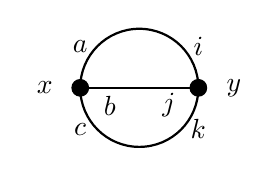
\begin{tikzpicture}[scale = 1.5, baseline=-1mm]
      % lines
      \draw[thick] (0, 0) node at (-.3, 0) {$x$} -- (1, 0) node at (1.3, 0) {$y$};
      \draw[thick] (0, 0) arc (180:0:.5);
      \draw[thick] (0, 0) arc (-180:0:.5);
      % nodes
      \draw[fill=black] (0, 0) circle (2pt);
      \draw[fill=black] (1, 0) circle (2pt);
      \node at (0, .35) {$a$};
      \node at (.25, -.15) {$b$};
      \node at (0, -.35) {$c$};
      \node at (1, .35) {$i$};
      \node at (0.75, -.15) {$j$};
      \node at (1, -.35) {$k$};
    \end{tikzpicture}
    \qquad \underset{
      \begin{aligned}
        i &\mapsto j \\ 
        j &\mapsto i
      \end{aligned}
      }{\cong} \qquad
    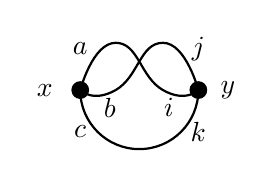
\begin{tikzpicture}[scale = 1.5, baseline=-1mm]
      % lines
      \draw[thick] plot[smooth, tension=1] coordinates { (0, 0) (.3, 0) (.7, .4) (1, 0) };
      \draw[thick] plot[smooth, tension=1] coordinates { (0, 0) (.3, .4) (.7, 0) (1, 0) };
      \draw[thick] (0, 0) arc (-180:0:.5);
      % nodes
      \draw[fill=black] (0, 0) circle (2pt);
      \draw[fill=black] (1, 0) circle (2pt);
      \node at (-.3, 0) {$x$};
      \node at (1.25, 0) {$y$};
      \node at (0, .35) {$a$};
      \node at (.25, -.15) {$b$};
      \node at (0, -.35) {$c$};
      \node at (1, .35) {$j$};
      \node at (0.75, -.15) {$i$};
      \node at (1, -.35) {$k$};
    \end{tikzpicture}
  \end{equation*}
  but no such graph isomorphism exists for between the following graphs.
  \begin{equation*}
  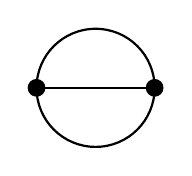
\begin{tikzpicture}[scale = 1.5, baseline=-1mm]
    % lines
    \draw[thick] (0, 0) -- (1, 0);
    \draw[thick] (0, 0) arc (180:0:.5);
    \draw[thick] (0, 0) arc (-180:0:.5);
    % nodes
    \draw[fill=black] (0, 0) circle (2pt);
    \draw[fill=black] (1, 0) circle (2pt);
  \end{tikzpicture}
  \qquad \ncong \qquad
  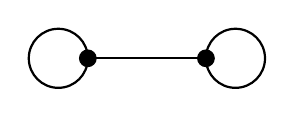
\begin{tikzpicture}[scale =1.5, baseline=-1mm]
    % lines
    \draw[thick] (0, 0) -- (1, 0);
    \draw[thick] (-.25, 0) circle (2.5mm);
    \draw[thick] (1.25, 0) circle (2.5mm);
    % nodes
    \draw[fill=black] (0, 0) circle (2pt);
    \draw[fill=black] (1, 0) circle (2pt);
  \end{tikzpicture}
  \end{equation*}
\end{example}

\begin{example}
  Consider homogeneous polynomials $P_d \in \Sym^d V^\vee$. We compute
  \begin{equation*}
    \bigavg{P_0(x)^{V_0} \dots P_D(x)^{V_D}}
    = \sum_{[\sigma]} \frac{|G|}{|\Aut \Gamma_\sigma|}
    (Q^{-1})^{\otimes m} \circ \sigma \circ (P_0^{V_0} \otimes \dots \otimes P_D^{V_D}) 
  \end{equation*}
  where
  \begin{equation*}
    |G| = \prod_{d = 0}^D (d!)^{V_d} V_d!.
  \end{equation*}
  We can rewrite this as
  \begin{equation*}
    \bigavg{P_0(x)^{V_0} \dots P_D(x)^{V_D}}
    = \biggl( \prod_{d = 0}^D (d!)^{V_d} V_d! \biggr)
    \sum_{\Gamma} \frac{1}{|\Aut \Gamma|} \Phi_{Q^{-1}, \{P_d\}} (\Gamma)
  \end{equation*}
  where we relabel the sum as being over graphs, to which we apply the following procedure.
  \begin{equation*}
    \begin{tikzcd}[sep=small]
    & \Phi_{Q^{-1}, \{{P_d}\}_{d = 0}^D} (\Gamma) \arrow[dr] \arrow[dl] & \\
      \text{label vertices } P_d \arrow[dr] & & \text{label edges } Q^{-1} \arrow[dl] \\
    & \text{contract $\Gamma$} &
  \end{tikzcd}
  \end{equation*}
\end{example}

\begin{example}
  For $\Psi \in \Sym^2 V^\vee$ we check that
  \begin{equation*}
    \bigavg{\Psi^3}
    = 8 \cdot 3! \biggl(
      \frac{1}{8 \cdot 3!} \hspace{-4mm}
      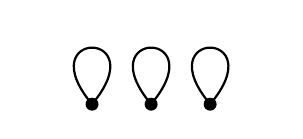
\begin{tikzpicture}[scale=2.5, baseline=2mm]
        % node
        \draw[fill=black] (0, 0) circle (.3mm);
        \draw[fill=black] (.3, 0) circle (.3mm);
        \draw[fill=black] (.6, 0) circle (.3mm);
        % lines
        \draw[thick] (0, 0) to[out=50, in=130, loop] (0, 0);
        \draw[thick] (.3, 0) to[out=50, in=130, loop] (.3, 0);
        \draw[thick] (.6, 0) to[out=50, in=130, loop] (.6, 0);
      \end{tikzpicture}
      \hspace{-4mm} + \frac{1}{8} \hspace{-3mm}
      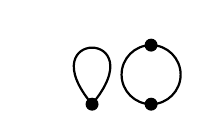
\begin{tikzpicture}[scale=2.5, baseline=2mm]
        % node
        \draw[fill=black] (0, 0) circle (.3mm);
        \draw[fill=black] (.3, 0) circle (.3mm);
        \draw[fill=black] (.3, .3) circle (.3mm);
        % lines
        \draw[thick] (0, 0) to[out=50, in=130, loop] (0, 0);
        \draw[thick] (.3, .15) circle (1.5mm);
      \end{tikzpicture}
      \hspace{1mm} + \frac{1}{6} \hspace{1mm}
      
\begin{tikzpicture}[scale=2.5, baseline=2mm]
        % node
        \draw[fill=black] (0, 0) circle (.3mm);
        \draw[fill=black] (.3, 0) circle (.3mm);
        \draw[fill=black] (.15, .3) circle (.3mm);
        % lines
        \draw[thick] (0, 0) to[out=120, in=180] (.15, .3);
        \draw[thick] (.15, .3) to[out=0, in=60] (.3, 0);
        \draw[thick] (0, 0) to[out=-60, in=240] (.3, 0);
      \end{tikzpicture}
    \biggr).
  \end{equation*}
\end{example}

% ── Perturbed Gaussian ────────────────────────────────────────────────
\subsection{Perturbed Gaussian}

We define a \textbf{perturbed} Gaussian integral
\begin{equation*}
  \int_{\Rbb^n}^\text{pert} \drm x \euler^{-\frac{1}{2} Q(x, x) + p(x)}
  = \biggl( \int_{\Rbb^n}^\text{pert} \drm x \euler^{\frac{1}{2} Q(x, x)} \biggr) \bigavg{\euler^{p(x)}}
\end{equation*}
where
\begin{equation*}
  p(x) = \sum_{d = 0}^D \frac{g_d P_d}{d!}, \qquad P_d \in \Sym^d V^\vee.
\end{equation*}
We write
\begin{equation*}
  \euler^{p(x)} 
  = \prod_{d = 0}^D \euler^{\frac{g_d P_d}{d!}}
  = \sum_{V_0, \dots, V_D} \biggl( \prod_{d = 0}^D \frac{g_d^{V_d}}{V_d! (d!)^{V_d}} \biggr)
  P_0(x)^{V_0} \dots P_D(x)^{V_D}
\end{equation*}
therefore
\begin{align*}
  \bigavg{\euler^{p(x)}}
  &= \sum_{V_0, \dots, V_D} g_0^{V_0} \dots g_D^{V_D}
  \sum_{\Gamma \in \mathsf{Graphs}_{V_0, \dots, V_D}}
  \frac{1}{|\Aut \Gamma|} \Phi_{Q^{-1}, \{P_d\}} (\Gamma) \\
  &= \underbrace{\sum_{\Gamma}}_{\substack{\text{sum over} \\ \text{all graphs}}} \frac{1}{|\Aut \Gamma|}
  \underbrace{\Phi_{Q^{-1}, \{g_d P_d\}}}_{\substack{\text{change labels} \\ P_d \, \mapsto \, g_d P_d}}.
\end{align*}

\begin{example}
  Let
  \begin{equation*}
    Q(x, x) = x^2, \qquad p(x) = \frac{\lambda}{4!} x^4.
  \end{equation*}
  In this case
  \begin{align*}
    I^p (\lambda)
    &= \int_{\Rbb^n}^\text{pert} \drm x \euler^{-\frac{1}{2} x^2 + \frac{\lambda}{4!} x^4} \\
    &= \sqrt{2 \pi} \biggl(
      1 + \frac{1}{8} \hspace{-2mm}
      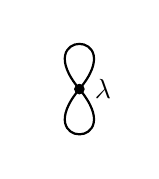
\begin{tikzpicture}[scale=2, baseline=-1mm]
        % node
        \draw[fill=black] (0, 0) circle (.3mm);
        \node at (.15, 0) {$\lambda$};
        % lines
        \draw[thick] (0, 0) to[out=50, in=130, loop] (0, 0);
        \draw[thick] (0, 0) to[out=230, in=-50, loop] (0, 0);
      \end{tikzpicture}
      + \frac{1}{8^2 2} \hspace{-2mm}
      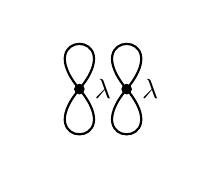
\begin{tikzpicture}[scale=2, baseline=-1mm]
        % node
        \draw[fill=black] (0, 0) circle (.3mm);
        \node at (.15, 0) {$\lambda$};
        \draw[fill=black] (.3, 0) circle (.3mm);
        \node at (.45, 0) {$\lambda$};
        % lines
        \draw[thick] (0, 0) to[out=50, in=130, loop] (0, 0);
        \draw[thick] (0, 0) to[out=230, in=-50, loop] (0, 0);
        \draw[thick] (.3, 0) to[out=50, in=130, loop] (.3, 0);
        \draw[thick] (.3, 0) to[out=230, in=-50, loop] (.3, 0);
      \end{tikzpicture}\\
    &\quad + \frac{1}{4! 2}
      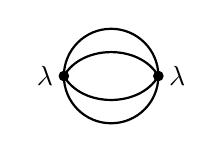
\begin{tikzpicture}[scale=2, baseline=-1mm]
        % node
        \draw[fill=black] (0, 0) circle (.3mm);
        \node at (-.12, 0) {$\lambda$};
        \draw[fill=black] (.6, 0) circle (.3mm);
        \node at (.72, 0) {$\lambda$};
        % lines
        \draw[thick] (.3, 0) circle (3mm);
        \draw[thick] (0, 0) to[out=60, in=120] (.6, 0);
        \draw[thick] (0, 0) to[out=-60, in=-120] (.6, 0);
      \end{tikzpicture}
    + \frac{1}{2^4} 
      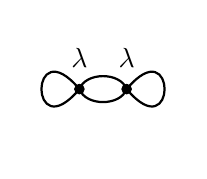
\begin{tikzpicture}[scale=2, baseline=-1mm]
        % node
        \draw[fill=black] (0, 0) circle (.3mm);
        \draw[fill=black] (.3, 0) circle (.3mm);
        \node at (0, .2) {$\lambda$};
        \node at (.3, .2) {$\lambda$};
        % lines
        \draw[thick] (0, 0) to[out=-130, in=130, loop] (0, 0);
        \draw[thick] (.3, 0) to[out=-50, in=50, loop] (.3, 0);
        \draw[thick] (0, 0) to[out=70, in=110] (.3, 0);
        \draw[thick] (0, 0) to[out=-70, in=-110] (.3, 0);
      \end{tikzpicture}
      + \Oscr \bigl(\lambda^3\bigr).
    \biggr) 
  \end{align*}
  The $n$-th coefficient of this series expansion is given by
  \begin{equation*}
    \sum_{\underbrace{\Gamma}_{\substack{n\text{ vertices} \\ \text{of valency } 4}}} \frac{1}{|\Aut \Gamma|}
    = \frac{(4n - 1)!!}{n! 4^n}.
  \end{equation*}
  This expression for $I^p (\lambda)$ has radius of convergence zero. Asymptotically, one can say that for all $N > 0$ there exists $M_N$ such that
  \begin{equation*}
    \biggl| I^p(\lambda) - \sqrt{2 \pi} \sum_{n=0}^N \lambda^n \frac{(4n - 1)!!}{n! 4^n} \biggr|
    \leq M_N |\lambda|^{N + 1}
  \end{equation*}
  for $\lambda < 0$ provided that $|\lambda|$ is sufficiently small.
\end{example}

% ── Connected graphs ──────────────────────────────────────────────────
\subsection{Connected graphs}

It can be useful to rewrite the usual expression in term of connected graphs. To achieve this, we decompose the sum with respect to the number of connected components of the graphs
\begin{align*}
  \sum_{\Gamma} \frac{1}{|\Aut \Gamma|} \Phi(\Gamma)
  &= \overbrace{\sum_{k = 0}^\infty}^{\substack{\text{connected}\\ \text{components}}}
  \sum_{\gamma_1, \dots, \gamma_k}
  \overbrace{\sum_{r_1, \dots, r_k = 1}^\infty}^{\text{valencies}}
  \biggl( \prod_{i=1}^k \frac{1}{r_i! |\Aut \gamma_i|} \biggr) \Phi(\gamma_1)^{r_1} \dots \Phi(\gamma_k)^{r_k} \\
  &= \underbrace{\prod_{\gamma \text{ connected}}}_{\substack{\text{finitely-many} \\ \text{nonzero valencies}}}
    \biggl( \sum_{r=0}^\infty \frac{1}{r! |\Aut \gamma|^r} \Phi(\gamma)^r \biggr) \\
  &= \prod_{\gamma \text{ connected}} \exp \biggl( \frac{1}{|\Aut \gamma|} \Phi(\gamma) \biggr) \\
  &= \exp \Biggl( \sum_{\gamma \text{ connected}} \frac{1}{|\Aut \gamma|} \Phi(\gamma) \Biggr).
\end{align*}

\begin{example}
  We can repeat the same computation summing on connected diagrams
  \begin{align*}
    I^p(\lambda)
    &= \sqrt{2 \pi} \exp \Biggl( 
      \frac{1}{8} \hspace{-2mm}
      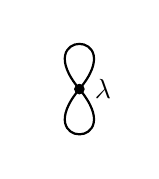
\begin{tikzpicture}[scale=2, baseline=-1mm]
        % node
        \draw[fill=black] (0, 0) circle (.3mm);
        \node at (.15, 0) {$\lambda$};
        % lines
        \draw[thick] (0, 0) to[out=50, in=130, loop] (0, 0);
        \draw[thick] (0, 0) to[out=230, in=-50, loop] (0, 0);
      \end{tikzpicture}
    + \frac{1}{4! 2}
    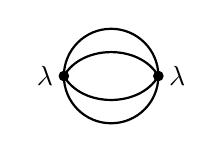
\begin{tikzpicture}[scale=2, baseline=-1mm]
      % node
      \draw[fill=black] (0, 0) circle (.3mm);
      \node at (-.12, 0) {$\lambda$};
      \draw[fill=black] (.6, 0) circle (.3mm);
      \node at (.72, 0) {$\lambda$};
      % lines
      \draw[thick] (.3, 0) circle (3mm);
      \draw[thick] (0, 0) to[out=60, in=120] (.6, 0);
      \draw[thick] (0, 0) to[out=-60, in=-120] (.6, 0);
    \end{tikzpicture}
    + \frac{1}{2^4} 
    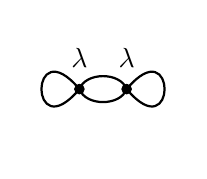
\begin{tikzpicture}[scale=2, baseline=-1mm]
      % node
      \draw[fill=black] (0, 0) circle (.3mm);
      \draw[fill=black] (.3, 0) circle (.3mm);
      \node at (0, .2) {$\lambda$};
      \node at (.3, .2) {$\lambda$};
      % lines
      \draw[thick] (0, 0) to[out=-130, in=130, loop] (0, 0);
      \draw[thick] (.3, 0) to[out=-50, in=50, loop] (.3, 0);
      \draw[thick] (0, 0) to[out=70, in=110] (.3, 0);
      \draw[thick] (0, 0) to[out=-70, in=-110] (.3, 0);
    \end{tikzpicture}
    + \Oscr \bigl(\lambda^3\bigr) \Biggr) \\
    &= \sqrt{2 \pi} \exp \biggl( \frac{\lambda}{8} + \frac{\lambda^2}{4!}
        + \frac{\lambda^2}{16} + \Oscr \bigl( \lambda^3 \bigr) \biggr) \\
    &= \sqrt{2 \pi} \biggl( 1 + \frac{\lambda}{8} + \frac{\lambda^2}{2 4!}
        + \frac{\lambda^2}{16} + \frac{\lambda^2}{ 8^2 2}
        + \Oscr \bigl( \lambda^3 \bigr) \biggr).
  \end{align*}
\end{example}

% ── Expectation value of perturbed Gaussian ───────────────────────────
\subsection{Expectation value of perturbed Gaussian}

To compute expectation values note that
\begin{align*}
  \bigavg{\Psi_1 \dots \Psi_r}_\text{pert}
  &= \frac{
    \int_{\Rbb^n}^\text{pert} \drm x
    \euler^{-\frac{1}{2} Q(x, x) + p(x)} \Psi_1(x) \dots \Psi_r (x)
  }{
    \int_{\Rbb^n}^\text{pert} \euler^{-\frac{1}{2} Q(x, x) + p(x)}
  }\\
  &= \frac{
    \bigavg{\euler^{p(x)} \Psi_1 \dots \Psi_r}
  }{
  \bigavg{\euler^{p(x)}}
  }
\end{align*}
where each term $\Psi_j$ is of the form
\begin{equation*}
  \Psi_j = \sum_{d \geq 0} \frac{1}{d!} \Psi_{j, d}
\end{equation*}
for $\Psi_{j, d}$ homogeneous polynomials of degree $d$, therefore
\begin{equation*}
  \bigavg{\euler^{p(x)} \Psi_1 \dots \Psi_r}
  = \frac{(2 \pi)^{\frac{n}{2}}}{\sqrt{\det Q}}
  \sum_{\Gamma} \frac{1}{|\Aut \Gamma|} \Psi(\Gamma)
\end{equation*}
where now we are summing over graphs $\Gamma$ colored by $\{0, \dots, r\}$ where each nonzero color appears \textit{exactly once}, and where $\Phi(\Gamma)$ encodes the following procedure.
\begin{equation*}
  \begin{tikzcd}
    & \Phi(\Gamma) \arrow[dl] \arrow[d] \arrow[dr] & \\
    \substack{\text{label } 0 \text{-colored}\\
      \text{vertices of valency } d \\
    \text{by } g_d P_d} \arrow[dr] &
    \substack{\text{label } j \text{-colored}\\
      \text{vertices of valency } d \\
      \text{by } \Psi_{j, d}} \arrow[d] &
    \substack{\text{label edges}\\
      \text{by } Q^{-1}} \arrow[dl] \\
    &\text{\scriptsize contract $\Gamma$}&
  \end{tikzcd}
\end{equation*}
